\documentclass[12pt]{article}

%\usepackage{algo}
\usepackage{tikz,fullpage,url,amssymb,amsmath,epsfig,color,xspace,alltt,mathtools}
\usetikzlibrary{shapes,chains,positioning}
\usepackage[pdftitle={CS 240 Assignment 3},%
pdfsubject={University of Waterloo, CS 240, Fall 2021},%
pdfauthor={MP}]{hyperref}
%\RequirePackage{pstricks,pst-node,pst-tree} % draw trees, requires using xetex
\newlength{\nodeLength}
\newcommand{\Node}{A}
\newcommand{\setnode}[1]{
	\settowidth{\nodeLength}{#1}
	\renewcommand{\Node}[1]{
		\Tcircle[name=#1]{\makebox[\nodeLength]{##1}}
	}
}
\setnode{99}

\newcommand{\ceil}[1]{\left\lceil #1 \right\rceil}
\newcommand{\floor}[1]{\left\lfloor #1 \right\rfloor}
\renewcommand{\thesubsection}{Problem \arabic{subsection}}

\begin{document}
	
	\begin{center}
		{\Large\bf Assignment 3 Problem 1}\\
		\vspace{3mm}
	\end{center}
	
	\definecolor{care}{rgb}{0,0,0}
	\def\question#1{\item[\bf #1.]}
	\def\part#1{\item[\bf #1)]}
	\newcommand{\pc}[1]{\mbox{\textbf{#1}}} % pseudocode
	
	
	
	%%%%%%%%%%%%%%%%%%%%%%%%%%%%%%%%%%%%%%%%%%%%%%%%%%%%%%%%%%%%%
	
	%%%%%%%%%%%%%%%%%%%%%%%%%%%%%%%%%%%%%%%%%%%%%%%%%%%%%%%%%%%%%
	%%% Problem 1
	\subsection{[0+2+2=4 marks]}
	
	\begin{enumerate}
		\part{a} {\bf Practice} (not worth any marks):  Starting with an empty AVL tree, insert the following keys in order: 27 99 17 28 42 16 1 2 4. \\
		
		You should obtain the AVL tree given in the next part.
		
		\part{b} Given the following AVL tree: \\
		Note: this tree shows balance factors instead of height.
		
		\begin{center}
			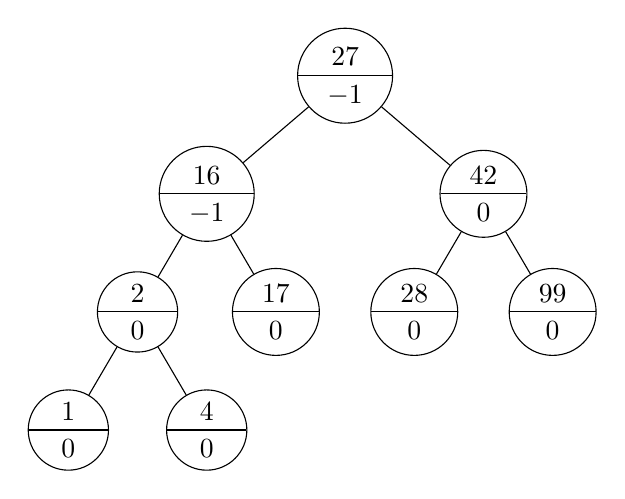
\begin{tikzpicture}[
				every node/.style = {draw, shape = circle split, grow = down},
				level 1/.style={sibling distance=100 pt},
				level 2/.style={sibling distance=50pt}]
				\node(z){$27$\nodepart{lower}$-1$}
				child{node{16\nodepart{lower}$-1$}
					child{node {2\nodepart{lower}$0$}
						child {node {1\nodepart{lower}$0$}}
						child {node {4\nodepart{lower}$0$}}}
					child{node {17\nodepart{lower}$0$}}
				}
				child{
					node{42\nodepart{lower}$0$}
					child{node {28\nodepart{lower}$0$}}
					child{node {99\nodepart{lower}$0$}}
				};
			\end{tikzpicture}
		\end{center}
		
		Insert the following keys in order:  8$^\star$, 22, 21, 18$^\star$.
		
		Show the resulting AVL trees with {\bf balance factors} (not height) for each node after the elements marked with star ($\star$) are inserted. \\
		Note: you should only show 2 trees.
		
		\part{c}  Consider the following AVL tree:
		\begin{center}
			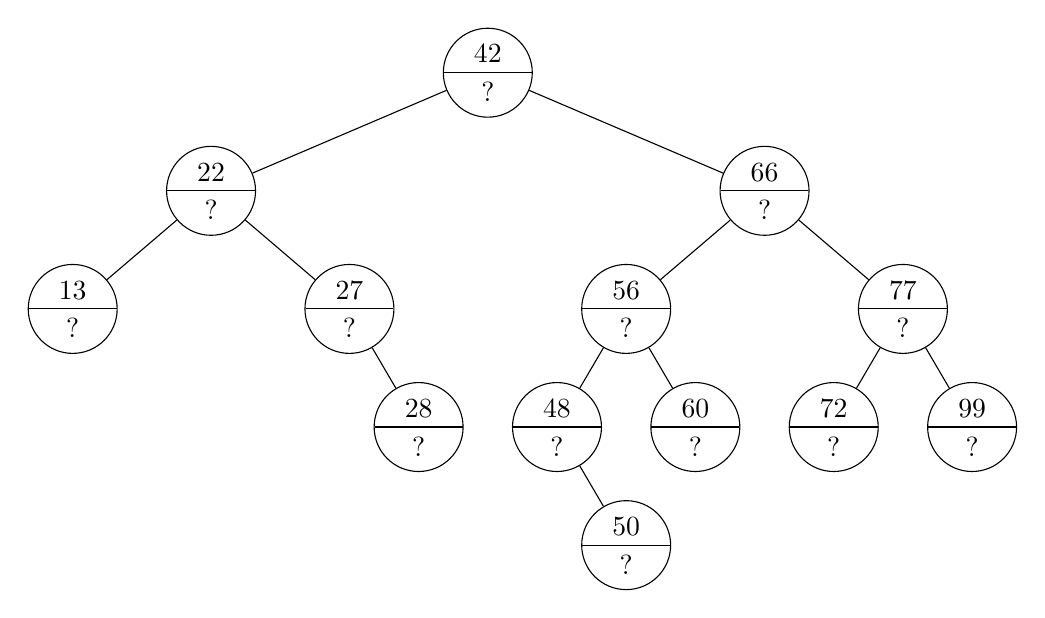
\begin{tikzpicture}[
				every node/.style = {draw, shape = circle split, grow = down},
				level 1/.style={sibling distance=200pt},
				level 2/.style={sibling distance=100pt},
				level 3/.style={sibling distance=50pt}]
				\node(z){$42$\nodepart{lower}$?$}
				child{node{22\nodepart{lower}$?$}
					child {node {13\nodepart{lower}$?$}}
					child {node {27\nodepart{lower}$?$}
						child[missing]
						child {node {28\nodepart{lower}$?$}}}}
				child {node {66\nodepart{lower}$?$}
					child {node {56\nodepart{lower}$?$}
						child {node {48\nodepart{lower}$?$}
							child[missing]
							child {node {50\nodepart{lower}$?$}}}
						child {node {60\nodepart{lower}$?$}}}
					child {node{77\nodepart{lower}$?$}
						child{node {72\nodepart{lower}$?$}}
						child{node {99\nodepart{lower}$?$}}}}
				;
			\end{tikzpicture}
		\end{center}
		
		Given the above tree, delete the following keys in order:
		
		\begin{center}
			66, 13$^\star$, 72, 77, 56$^\star$, 42$^\star$ 
		\end{center}
		
		Show the resulting AVL trees with {\bf balance factors} (not height) for each node after the elements marked with star ($\star$) are deleted.  
		If you have a choice of which element to move up, pick the inorder successor. \\
		Note: you should only show 3 trees.
		
	\end{enumerate}
	
	\begin{enumerate}
		\part{b} Solution:
		\begin{center}
			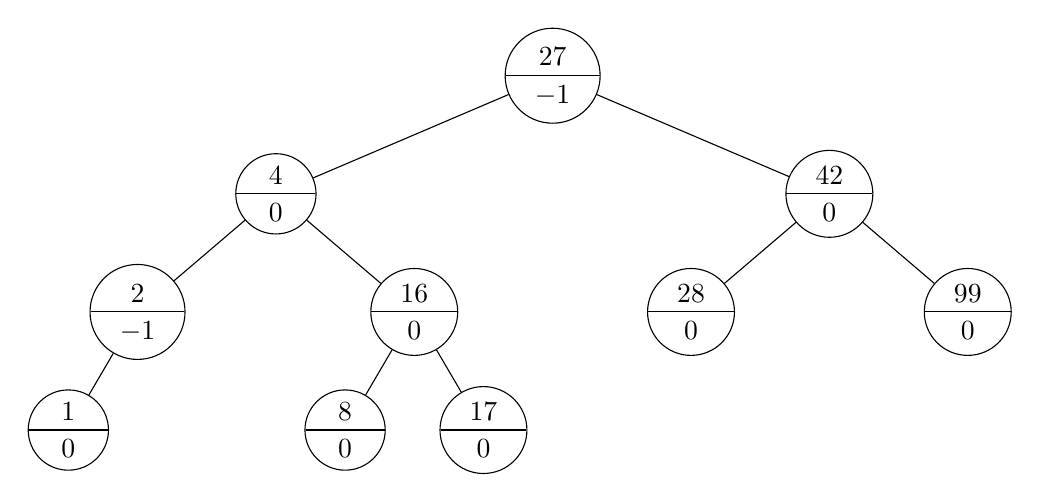
\begin{tikzpicture}[
				every node/.style = {draw, shape = circle split, grow = down},
				level 1/.style={sibling distance=200pt},
				level 2/.style={sibling distance=100pt},
				level 3/.style={sibling distance=50pt}]
				\node(z){$27$\nodepart{lower}$-1$}
				child{node {4\nodepart{lower}$0$}
					child{node {2\nodepart{lower}$-1$}
						child {node {1\nodepart{lower}$0$}}
						child [missing]}
					child{node {16\nodepart{lower}$0$}
						child {node {8\nodepart{lower}$0$}}
						child {node {17\nodepart{lower}$0$}}}
				}
				child{node {42\nodepart{lower}$0$}
					child{node {28\nodepart{lower}$0$}}
					child{node {99\nodepart{lower}$0$}}
				};
			\end{tikzpicture}
			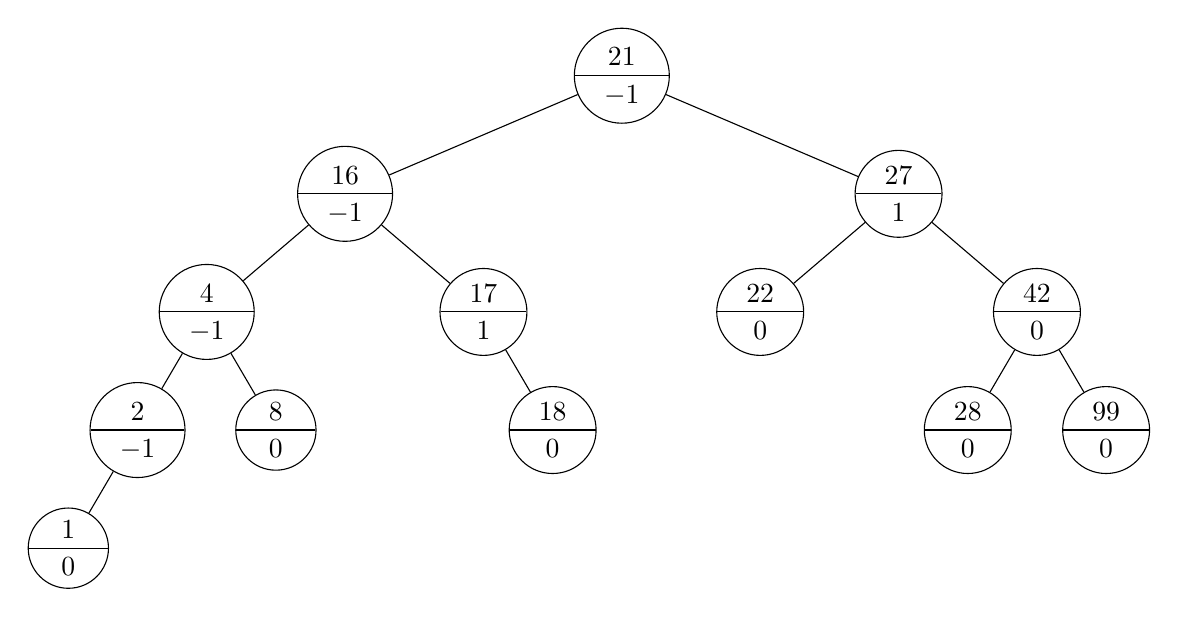
\begin{tikzpicture}[
				every node/.style = {draw, shape = circle split, grow = down},
				level 1/.style={sibling distance=200pt},
				level 2/.style={sibling distance=100pt},
				level 3/.style={sibling distance=50pt}]
				\node(z){$21$\nodepart{lower}$-1$}
				child{node {16\nodepart{lower}$-1$}
					child{node {4\nodepart{lower}$-1$}
						child {node {2\nodepart{lower}$-1$}
							child {node {1\nodepart{lower}$0$}}
							child [missing]}
						child {node {8\nodepart{lower}$0$}}}
					child{node {17\nodepart{lower}$1$}
						child [missing]
						child {node {18\nodepart{lower}$0$}}}
				}
				child{node {27\nodepart{lower}$1$}
					child{node {22\nodepart{lower}$0$}}
					child{node {42\nodepart{lower}$0$}
						child {node {28\nodepart{lower}$0$}}
						child {node {99\nodepart{lower}$0$}}}
				};
			\end{tikzpicture}
		\end{center}
	
	\part{c} Solution:
	\begin{center}
		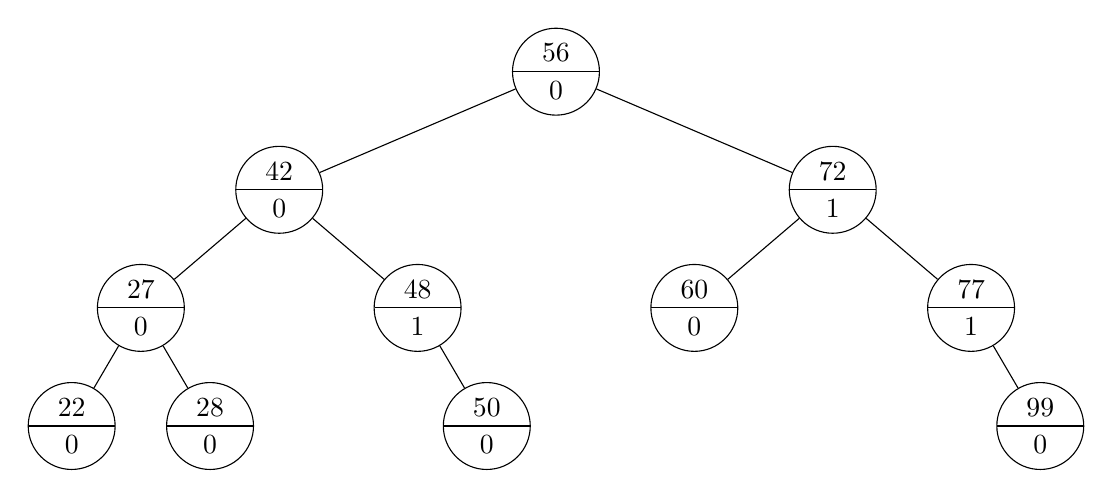
\begin{tikzpicture}[
			every node/.style = {draw, shape = circle split, grow = down},
			level 1/.style={sibling distance=200pt},
			level 2/.style={sibling distance=100pt},
			level 3/.style={sibling distance=50pt}]
			\node(z){$56$\nodepart{lower}$0$}
			child{node{42\nodepart{lower}$0$}
				child {node {27\nodepart{lower}$0$}
					child {node {22\nodepart{lower}$0$}}
					child {node {28\nodepart{lower}$0$}}}
				child {node {48\nodepart{lower}$1$}
					child [missing]
					child {node {50\nodepart{lower}$0$}}}}
			child {node {72\nodepart{lower}$1$}
				child {node {60\nodepart{lower}$0$}}
				child {node {77\nodepart{lower}$1$}
					child[missing]
					child{node {99\nodepart{lower}$0$}}}}
			;
		\end{tikzpicture}
		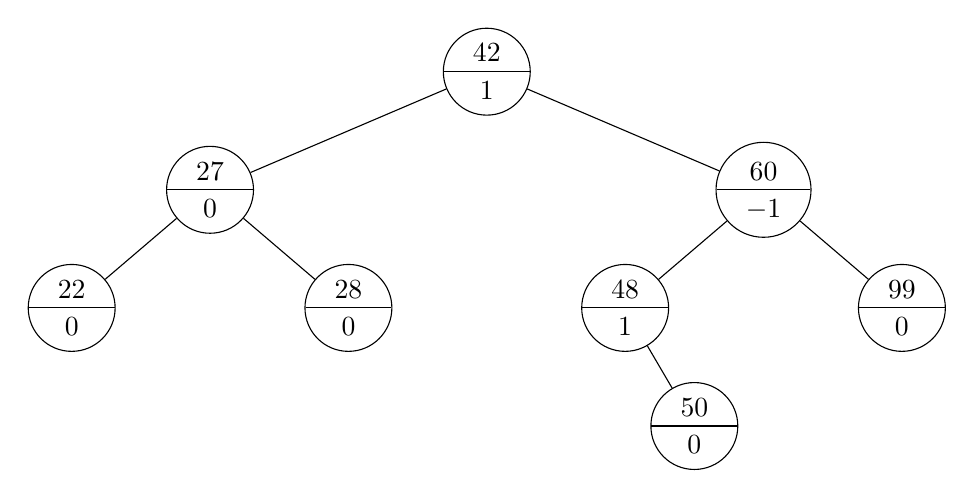
\begin{tikzpicture}[
			every node/.style = {draw, shape = circle split, grow = down},
			level 1/.style={sibling distance=200pt},
			level 2/.style={sibling distance=100pt},
			level 3/.style={sibling distance=50pt}]
			\node(z){$42$\nodepart{lower}$1$}
			child{node{27\nodepart{lower}$0$}
				child {node {22\nodepart{lower}$0$}}
				child {node {28\nodepart{lower}$0$}}}
			child {node {60\nodepart{lower}$-1$}
				child {node {48\nodepart{lower}$1$}
					child [missing]
					child {node {50\nodepart{lower}$0$}}}
				child {node {99\nodepart{lower}$0$}}}
			;
		\end{tikzpicture}
		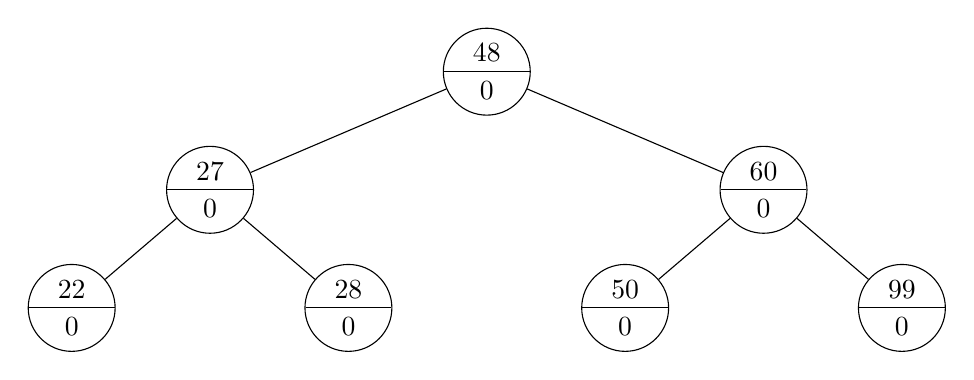
\begin{tikzpicture}[
			every node/.style = {draw, shape = circle split, grow = down},
			level 1/.style={sibling distance=200pt},
			level 2/.style={sibling distance=100pt},
			level 3/.style={sibling distance=50pt}]
			\node(z){$48$\nodepart{lower}$0$}
			child{node{27\nodepart{lower}$0$}
				child {node {22\nodepart{lower}$0$}}
				child {node {28\nodepart{lower}$0$}}}
			child {node {60\nodepart{lower}$0$}
				child {node {50\nodepart{lower}$0$}}
				child {node {99\nodepart{lower}$0$}}}
			;
		\end{tikzpicture}
	\end{center}
	
	\end{enumerate}
	%%%%%%%%%%%%%%%%%%%%%%%%%%%%%%%%%%%%%%%%%%%%%%%%%%%%%%%%%%%%%
\end{document}